Il filtro più importante è il Gaussian Blur, che prende in input: l’immagine filtrata dal black hat, un kernel (standard 5x5, che può essere eventualmente modificato con valori positivi dispari), una deviazione standard del kernel sigmaX e una sigmaY, nel nostro caso entrambe settate a 0 per farle calcolare automaticamente dalla funzione sulla base dei valori del kernel. 

\begin{minted}
  [
    xleftmargin=\parindent,
    framesep=2mm,
    baselinestretch=1.2,  
    fontsize=\footnotesize,
    linenos
  ]
  {python}
  
  final_img = cv2.GaussianBlur(bottom_hat_filtered, (5, 5), 0)   
  \end{minted}
  

In termini di elaborazione delle immagini, eventuali spigoli netti vengono uniformati, riducendo al minimo le sfocature. In questo caso l’utilità di questo filtro è quella di “pulire” ulteriormente l’immagine dell’occhio, semplificando la successiva identificazione della pupilla e,soprattutto, dell’iride.

\begin{figure}[t]
  \centering
  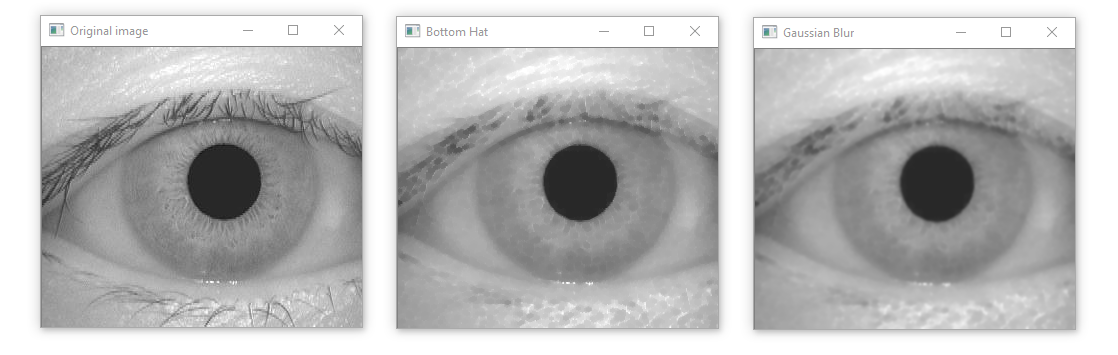
\includegraphics[width=1.0\textwidth]{gaussian_blur.png}
  \caption{Risultato dell'applicazione del Gaussian Blur dopo il filtro bottom hat}
\end{figure}
